\documentclass[11pt]{beamer}
\usetheme{Boadilla}
\usepackage[utf8]{inputenc}
\usepackage{amsmath}
\usepackage{amsfonts}
\usepackage{amssymb}
\usepackage{listings}
\usepackage{color}

\definecolor{dkgreen}{rgb}{0,0.6,0}
\definecolor{gray}{rgb}{0.5,0.5,0.5}
\definecolor{mauve}{rgb}{0.58,0,0.82}

\lstset{frame=tb,
  language=c++,
  aboveskip=3mm,
  belowskip=3mm,
  showstringspaces=false,
  columns=flexible,
  basicstyle={\small\ttfamily},
  numbers=none,
  numberstyle=\tiny\color{gray},
  keywordstyle=\color{blue},
  commentstyle=\color{dkgreen},
  stringstyle=\color{mauve},
  breaklines=true,
  breakatwhitespace=true,
  tabsize=3
}
\author{From the winter school}
\title{The JetScape Computational framework}
%\setbeamercovered{transparent} 
%\setbeamertemplate{navigation symbols}{} 
%\logo{} 
%\institute{} 
\date{\today} 

%\subject{} 
\begin{document}

\begin{frame}
\titlepage
\end{frame}

%\begin{frame}
%\tableofcontents
%\end{frame}

\begin{frame}
\begin{overprint}
\onslide<1> Modules: Hard process, nuclear initial condition, one/more transport model, hydro information, hadronization.
\onslide<2> Many modules require data / function calls from the others.
\end{overprint}
\begin{center}
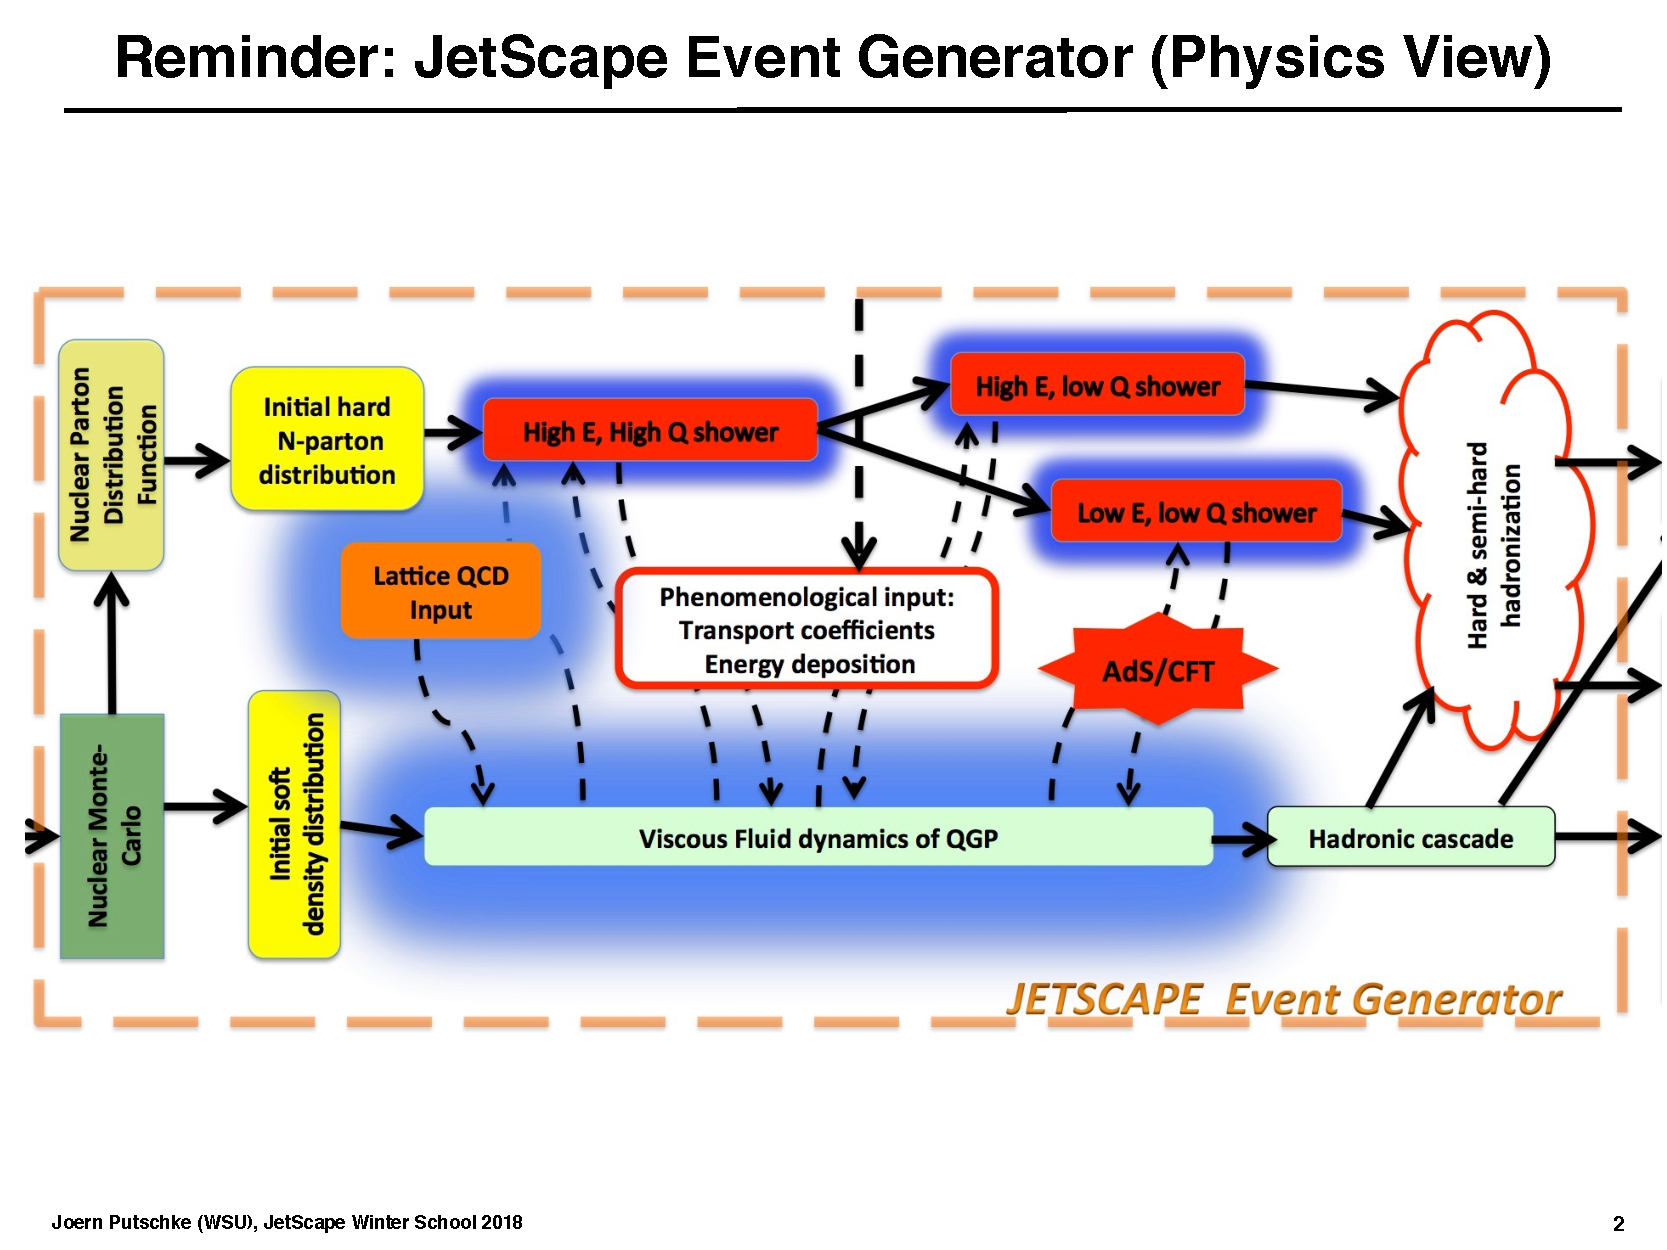
\includegraphics[width=0.9\textwidth]{./talks/p3.pdf}
\end{center}
\end{frame}

\begin{frame}
A jetscape object / environment that handles data feeding / collection; communication between modules; init and exec of each module, etc.
\begin{center}
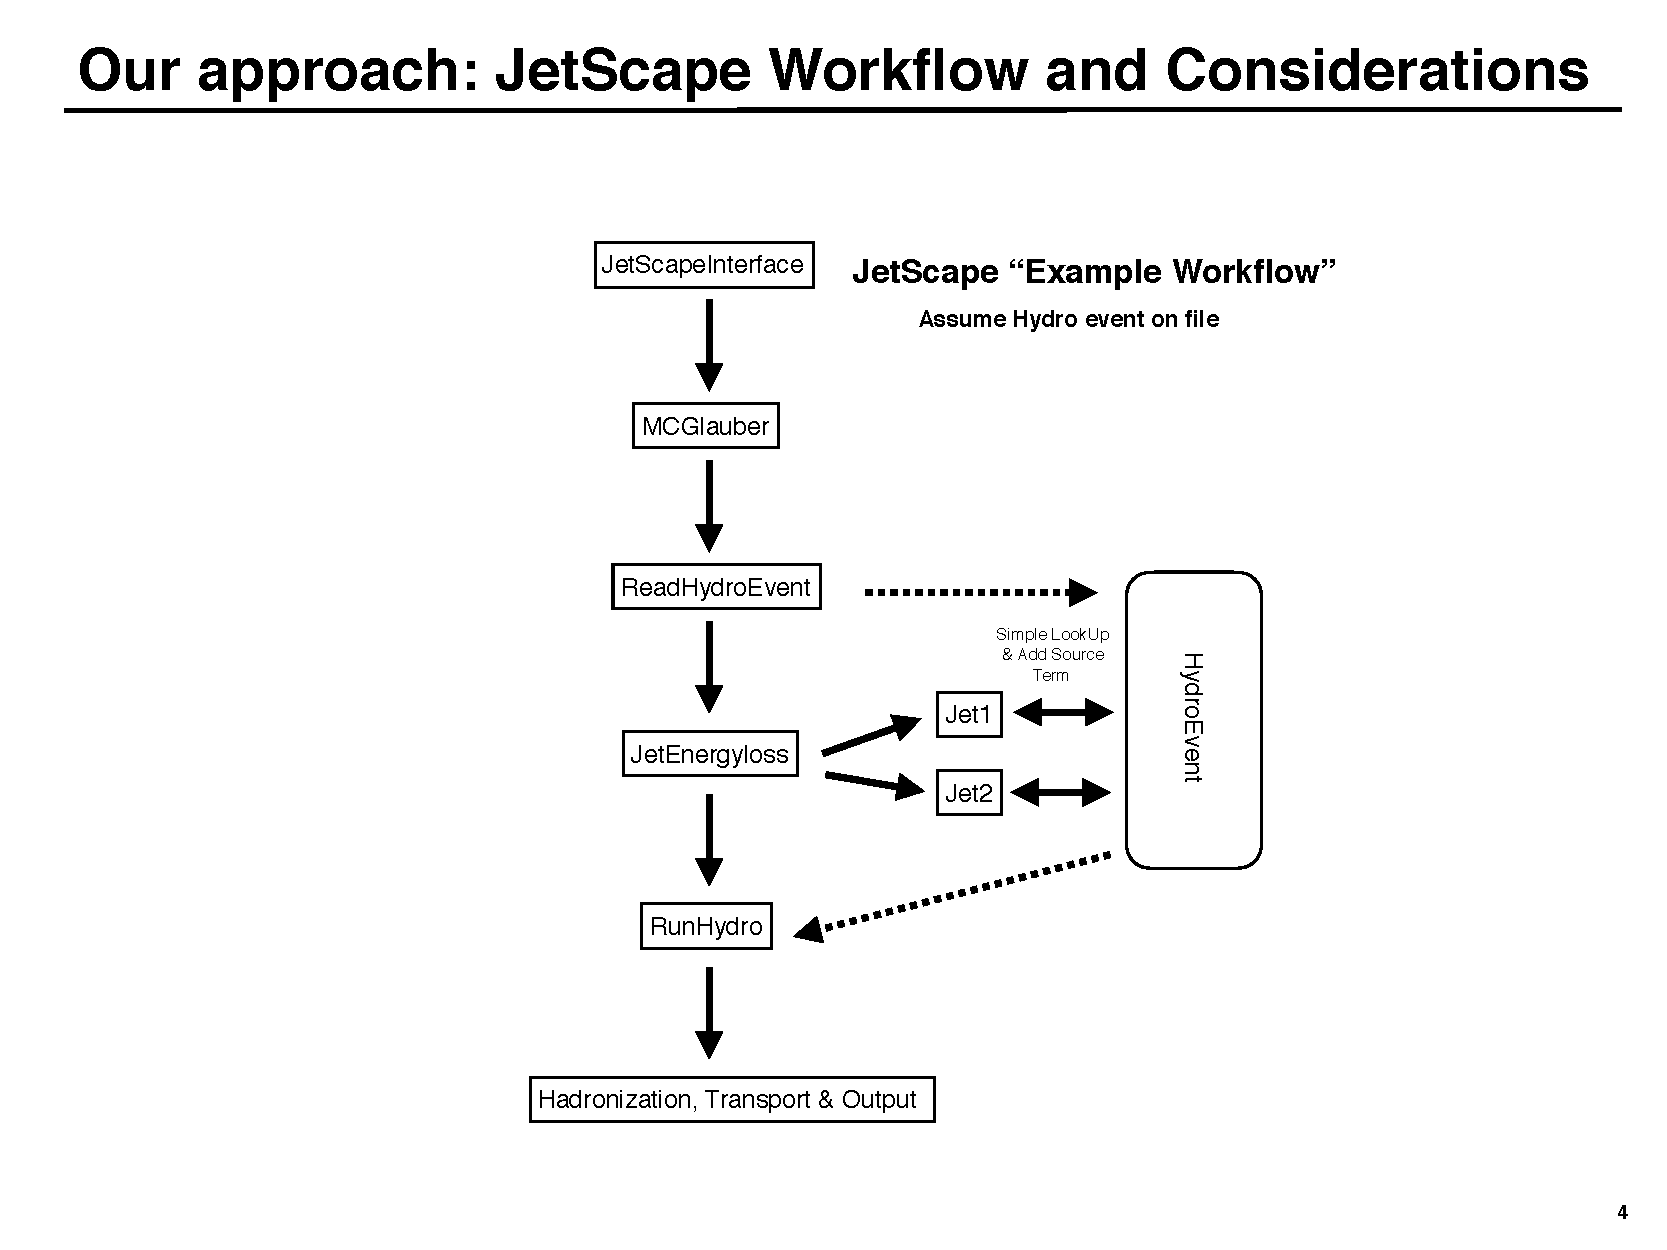
\includegraphics[width=0.95\textwidth]{./talks/p5.pdf}
\end{center}
\end{frame}

\begin{frame}
\begin{overprint}
\onslide<1> Each module appears as a task in the work-flow. Jetscape object executes the tasks and handles communications. 
\onslide<2> Users only focus on implementing physics.
\end{overprint}
\begin{center}
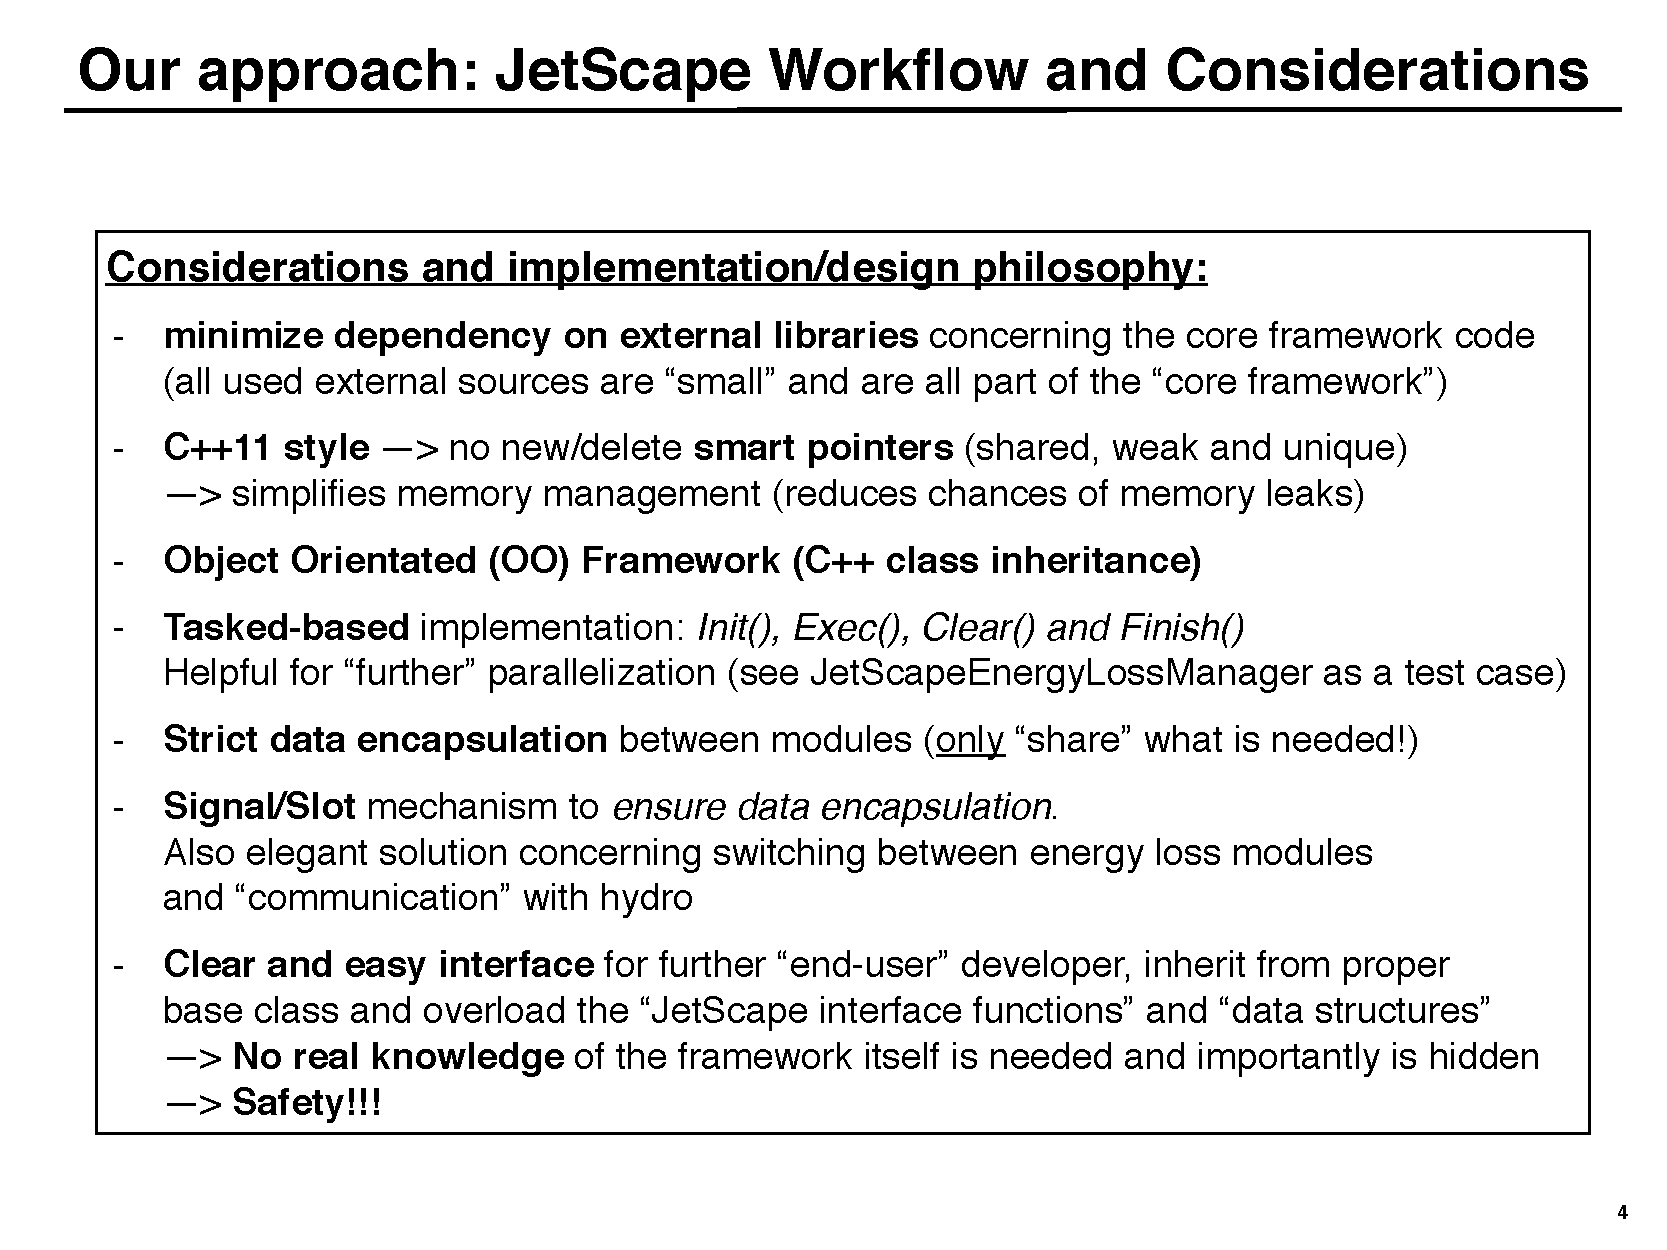
\includegraphics[width=0.95\textwidth]{./talks/p6.pdf}
\end{center}
\end{frame}

\begin{frame}
\begin{columns}
\begin{column}{0.8\textwidth}
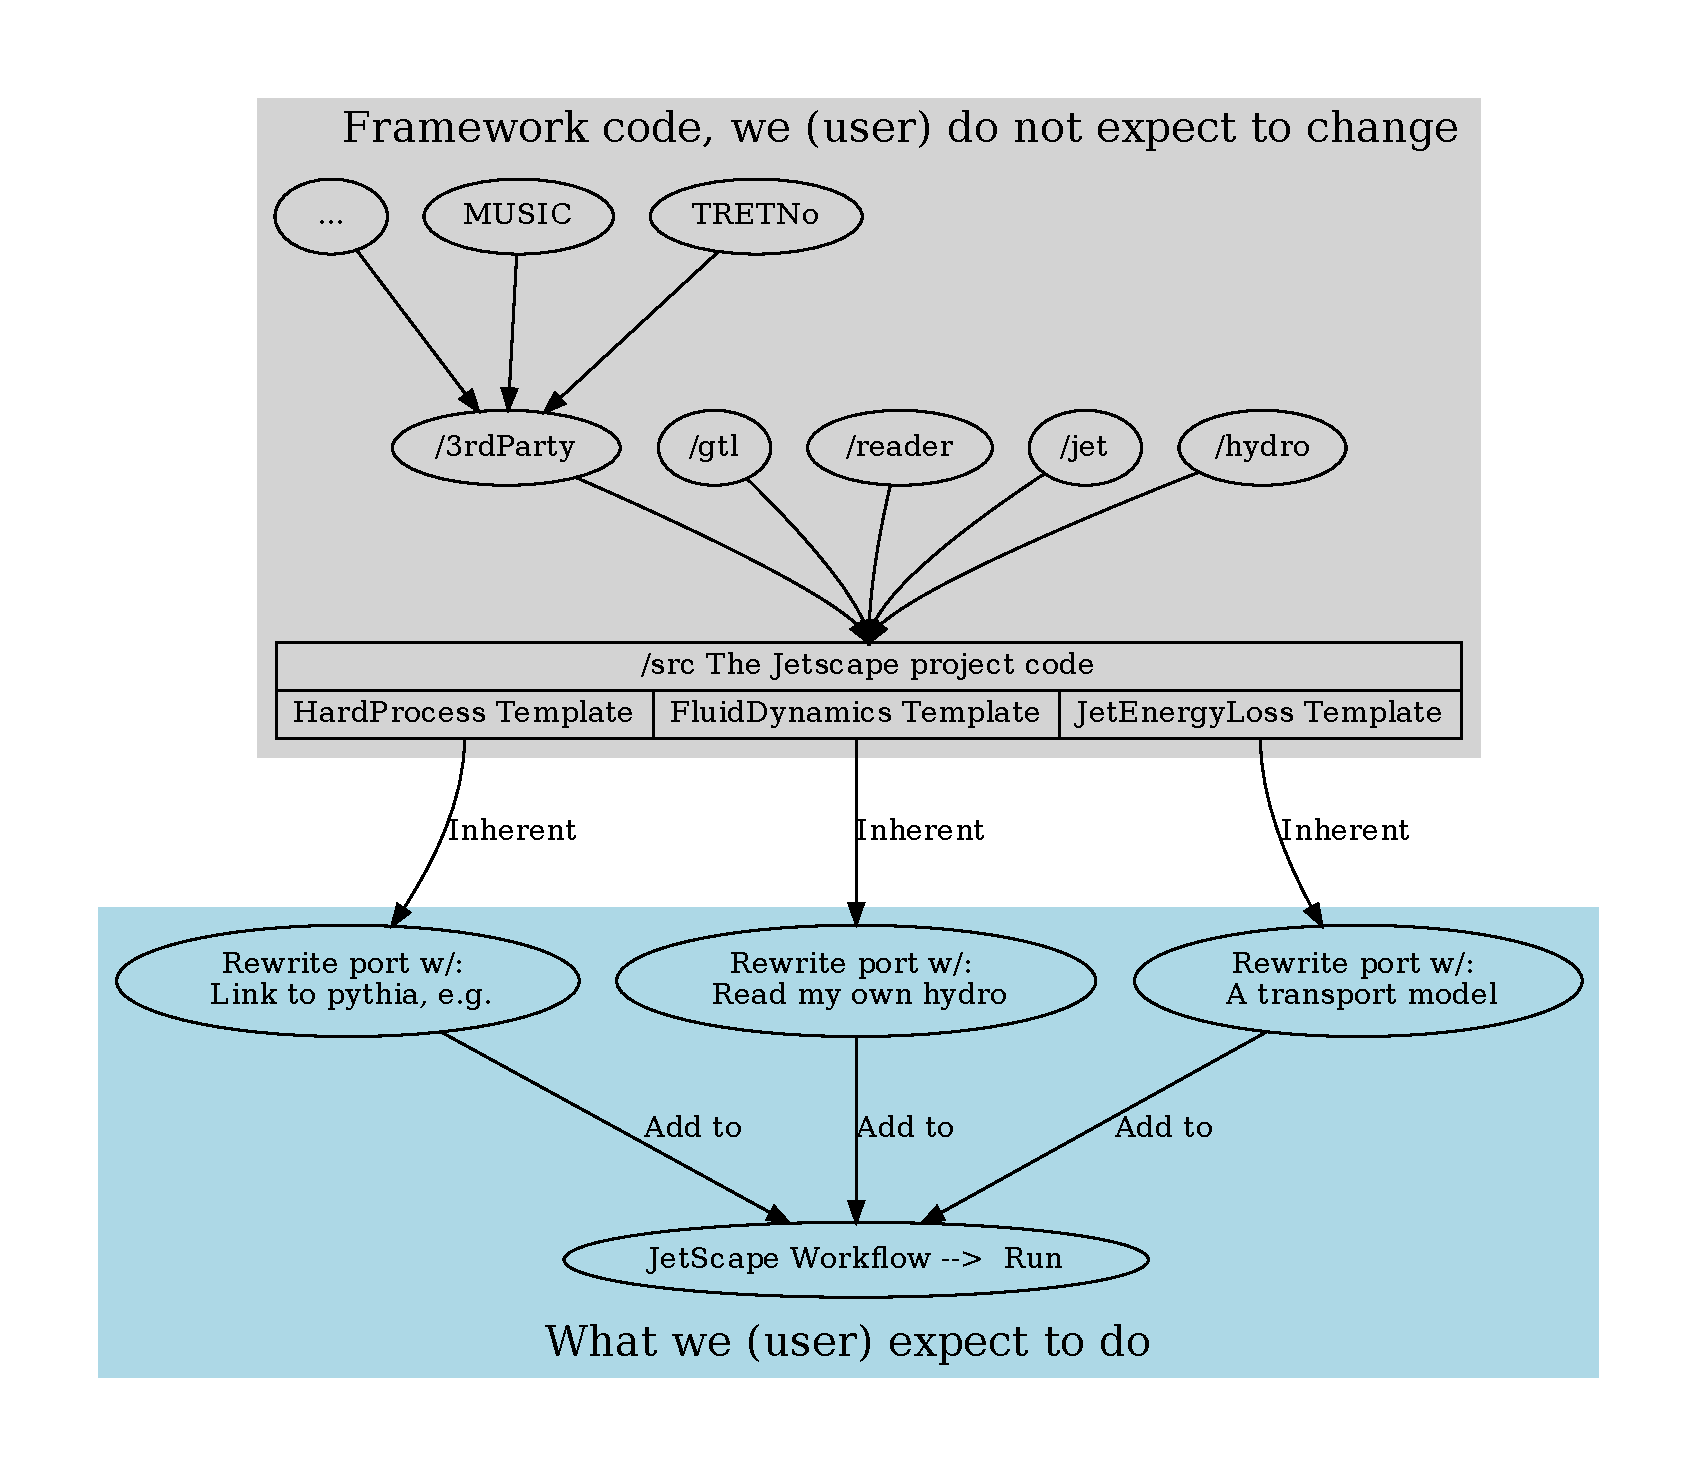
\includegraphics[width=\textwidth]{./framework.pdf}
\end{column}
\begin{column}{0.2\textwidth}
Framework code defines base class of phy modules.\\
\vspace{.5cm}
A template we can fill in our phy models.\\
\vspace{.5cm}
Duplicate the template and implement interface functions, e.g.\\
DoEnergyLoss()\\
GetHydroCell()
\end{column}
\end{columns}
\end{frame}

\begin{frame}
Here, the PGun, Brick, JetScapeWriterAscii, Matter and Martini are also user implemented modules based on corresponding jetscape templates.
\begin{center}
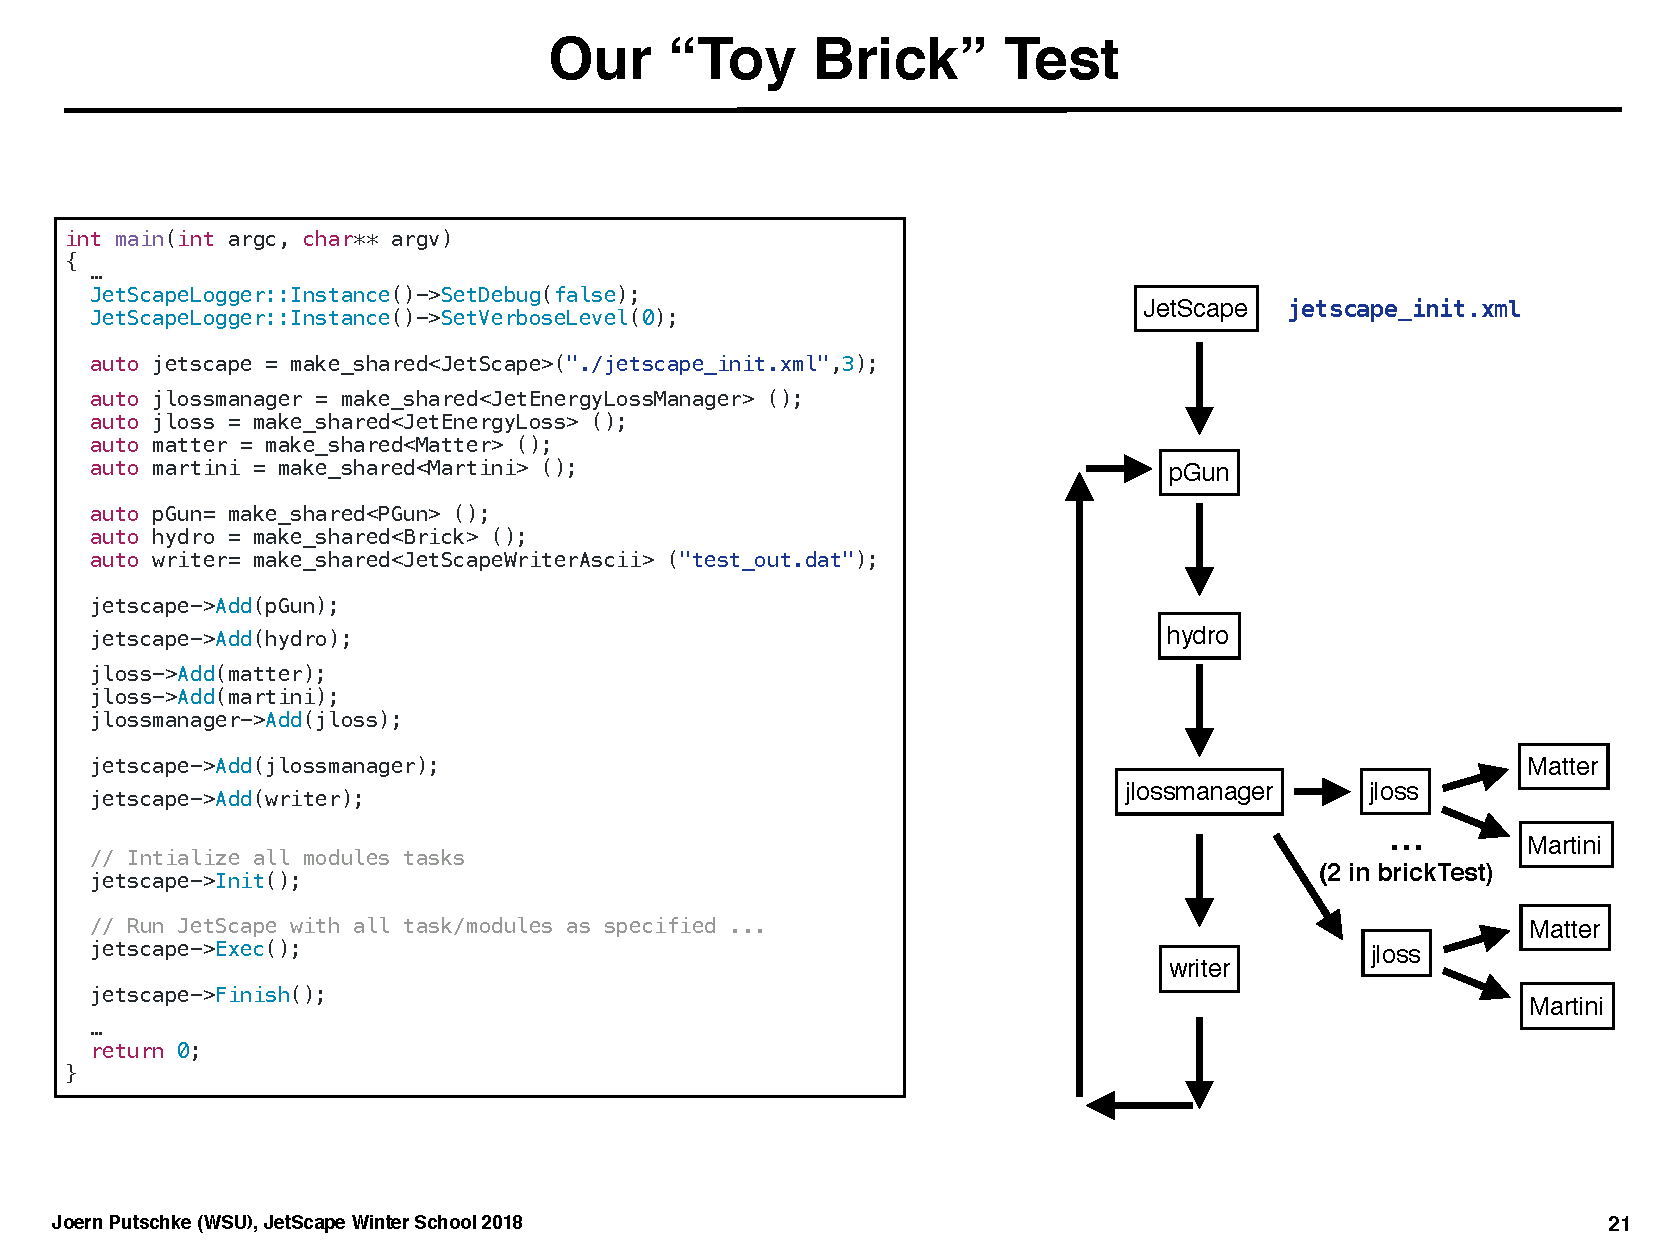
\includegraphics[width=0.9\textwidth]{./talks/p38.pdf}
\end{center}
\end{frame}

\begin{frame}
Then, add instances of user modules to the jetscape workflow. It will know when to execute each module and where to find the required data.
\begin{center}
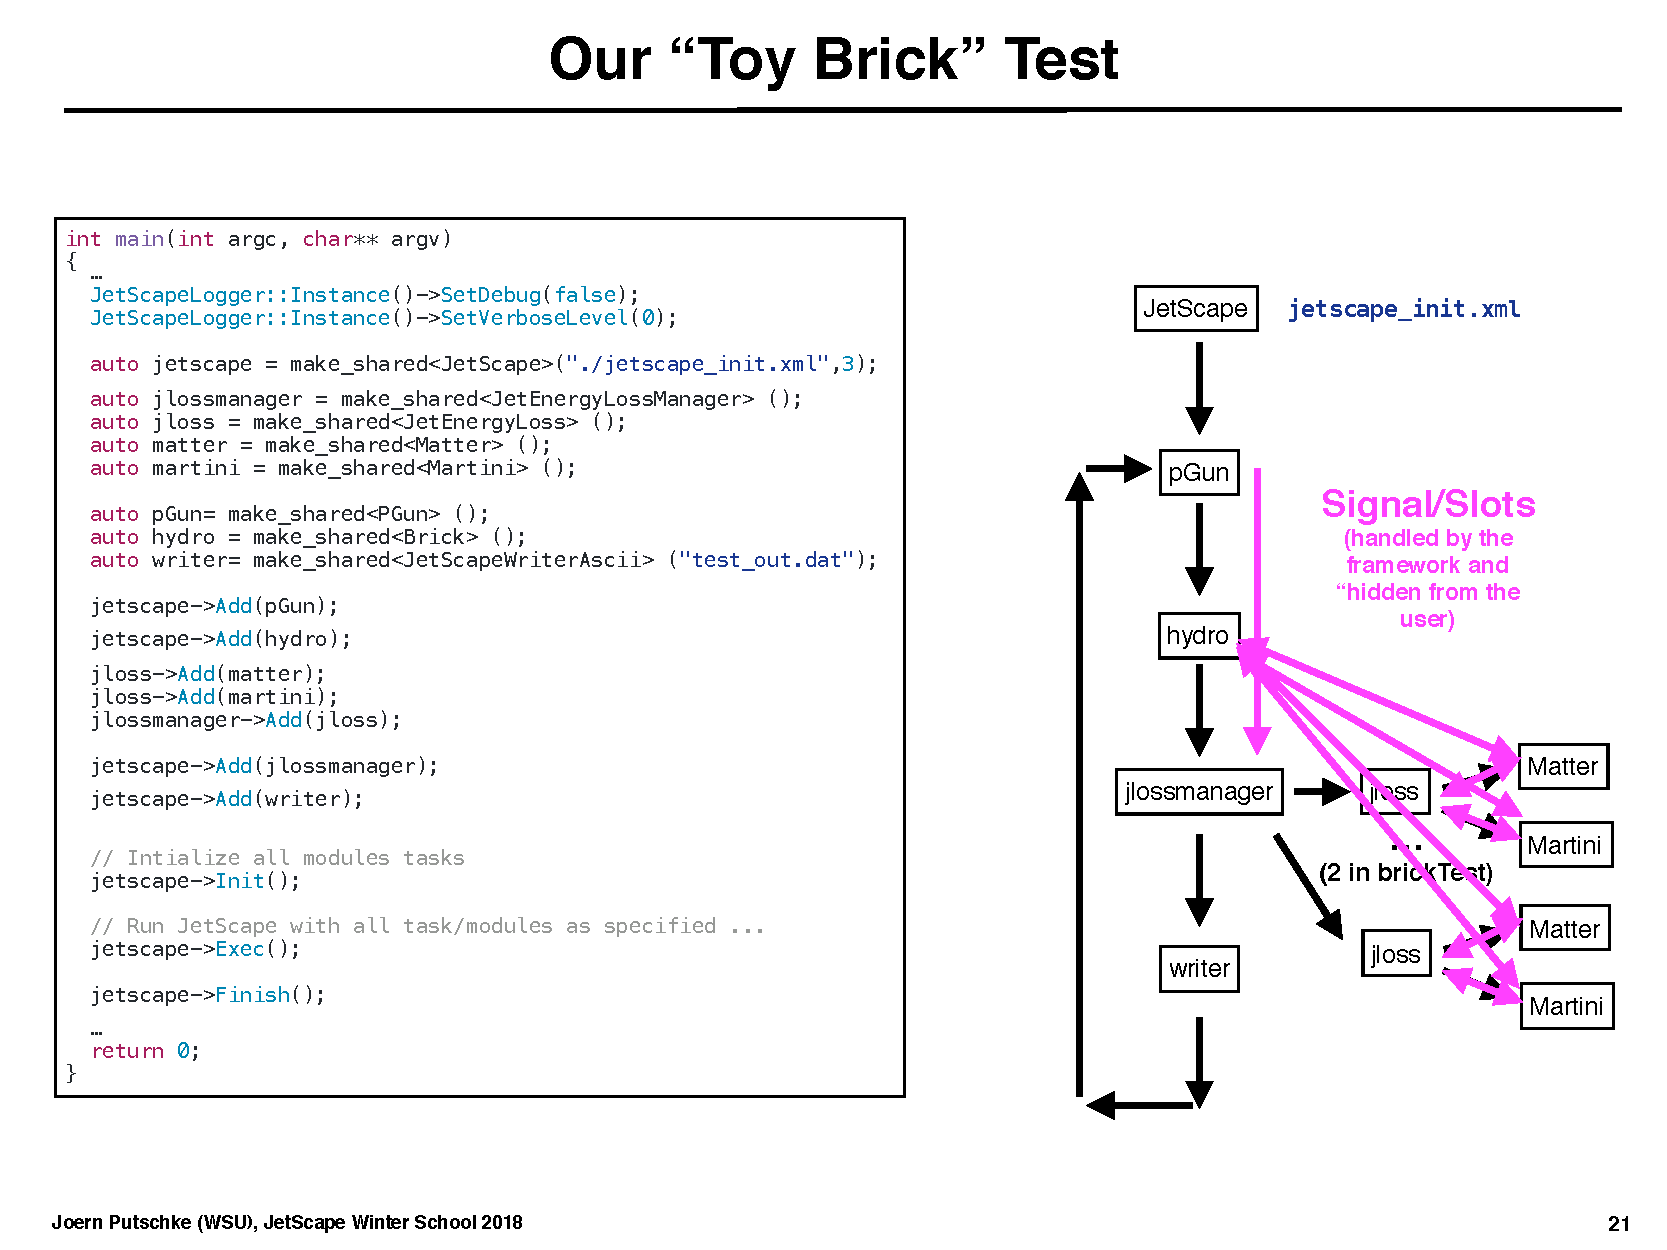
\includegraphics[width=0.9\textwidth]{./talks/p39.pdf}
\end{center}
\end{frame}

\begin{frame}
Combine different transport models is easy in this framework.
\begin{center}
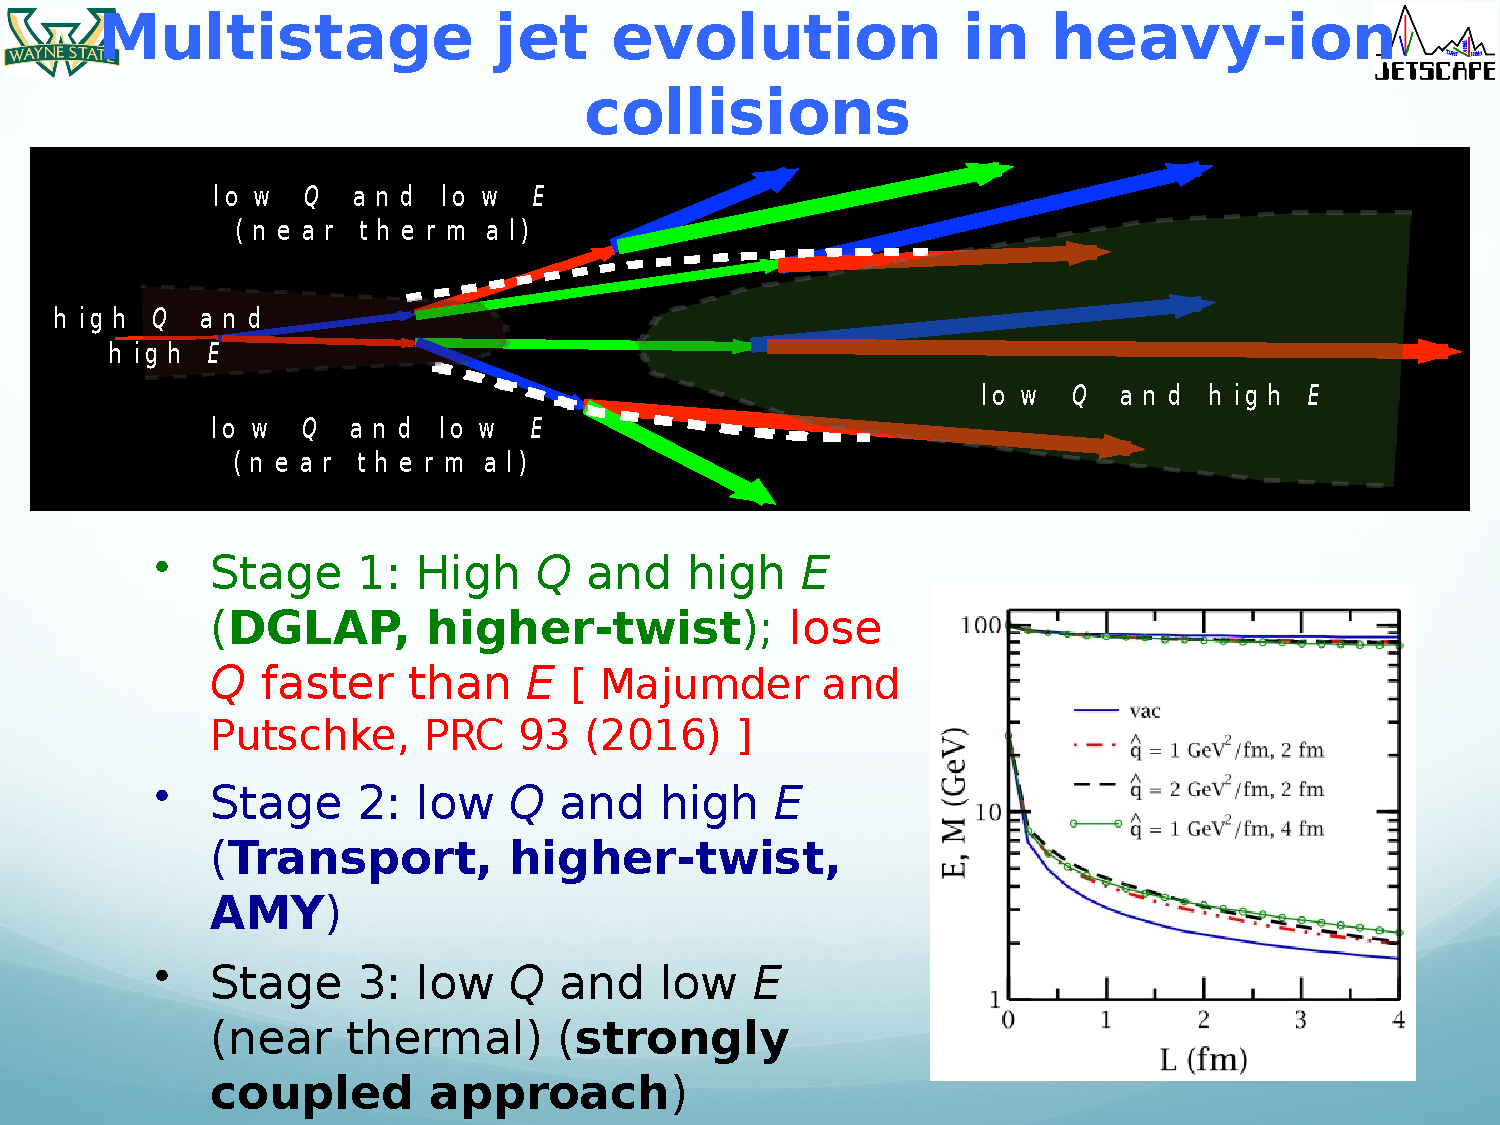
\includegraphics[width=0.9\textwidth]{./talks/s25.pdf}
\end{center}
\end{frame}

\begin{frame}[fragile]{"Easy" combination of multiple transport models}
For example:
\begin{itemize}
\item Matter handles parton evolution at large virtuality ($Q > 1$ GeV e.g.)
\item Martini / LBT (rate equations) apply at low virtuality.
\end{itemize}
In JetScape framework code, this is simply:
\begin{lstlisting}
...
jloss->Add(matter) // Matter check Q; only updates high Q partons
jloss->Add(martini) // Martini only updates low Q partons

jlossmanager->Add(joss)
jetscape->Add(jlossmanager)
jetscape->Init()
jetscape->Exec() // For each time step, jetscape calls matter followed by martini, and then next time step and so on...
...
\end{lstlisting}
The jetscape object will feed and collect the input/output parton data from the transport module. 
\end{frame}

\begin{frame}{Data are stored in trees}
\begin{itemize}
\item All the branchings, scatterings, of partons in jet are stored in a tree structure. One can reconstruct the whole time evolution.
\item User can also define new writers to output wanted info.
\item Jetscape also provides output to ".xml" format $\rightarrow$ visualization.\\
\end{itemize}

\end{frame}

\begin{frame}{Visualization tool}

\begin{overprint}
\onslide<1> Matter + Martini
\onslide<2> Matter
\onslide<3> Martini
\end{overprint}

\begin{center}
\begin{figure}
\begin{overprint}
\onslide<1>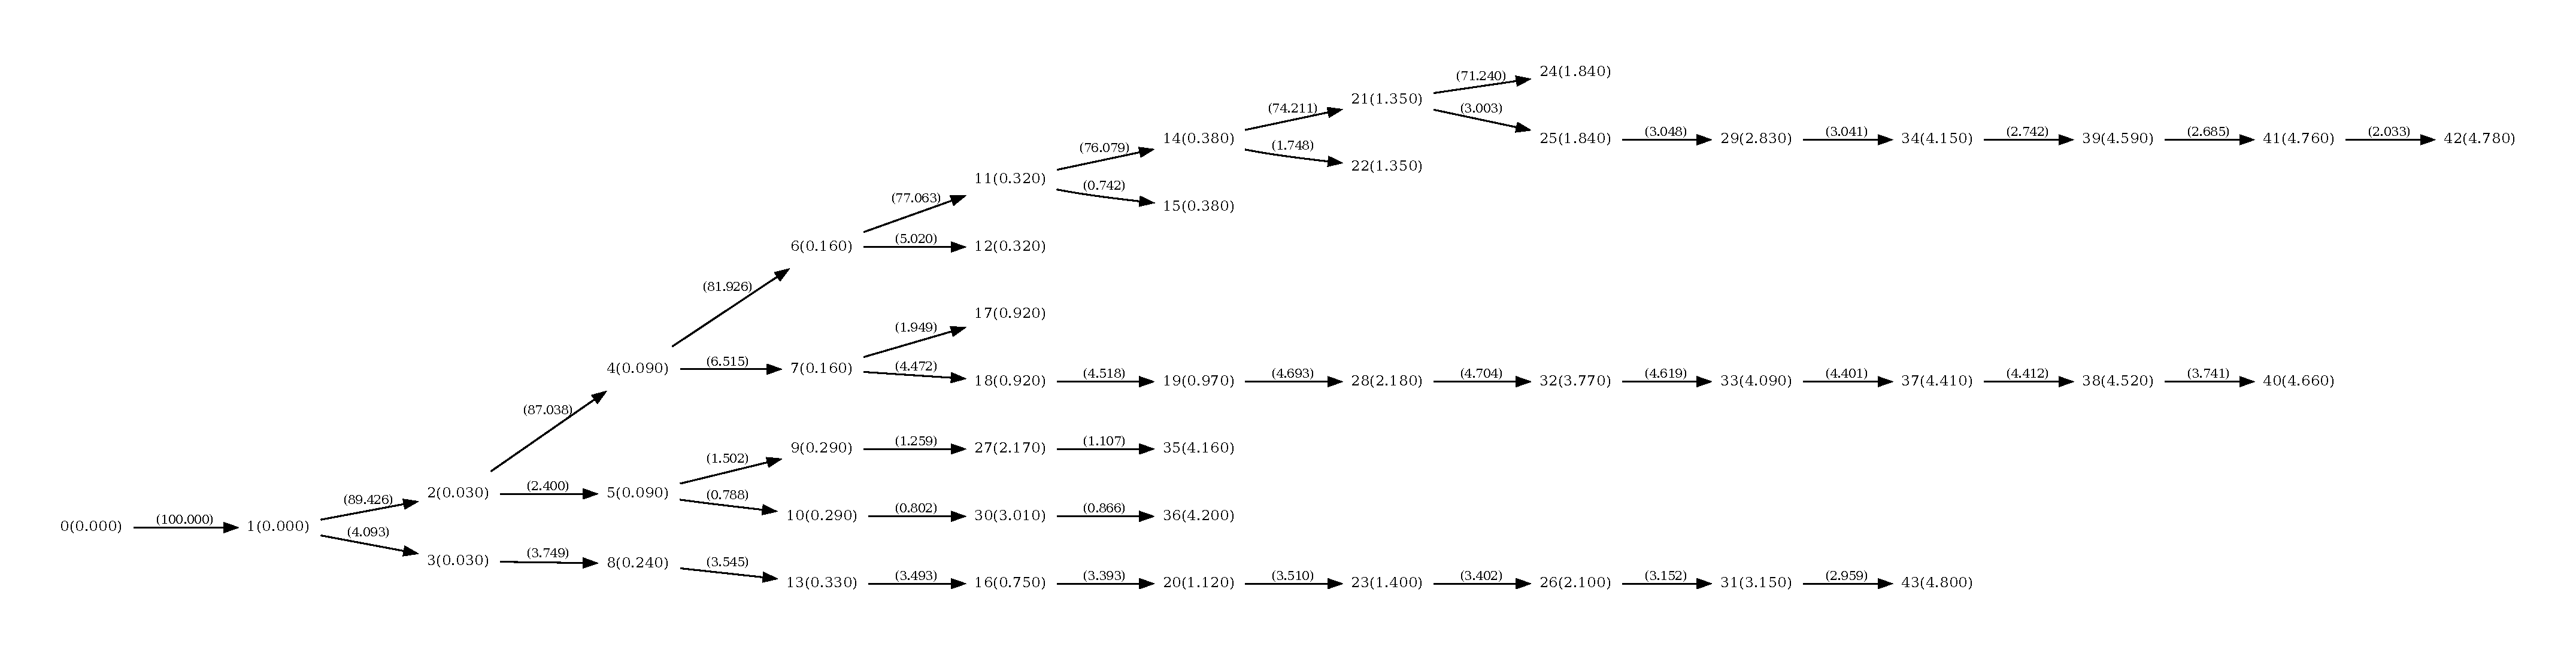
\includegraphics[width=1.8\textwidth]{./sample_jet_graph/graph-Matter-Martini/Jet_Matter_Martini.pdf}
\onslide<2>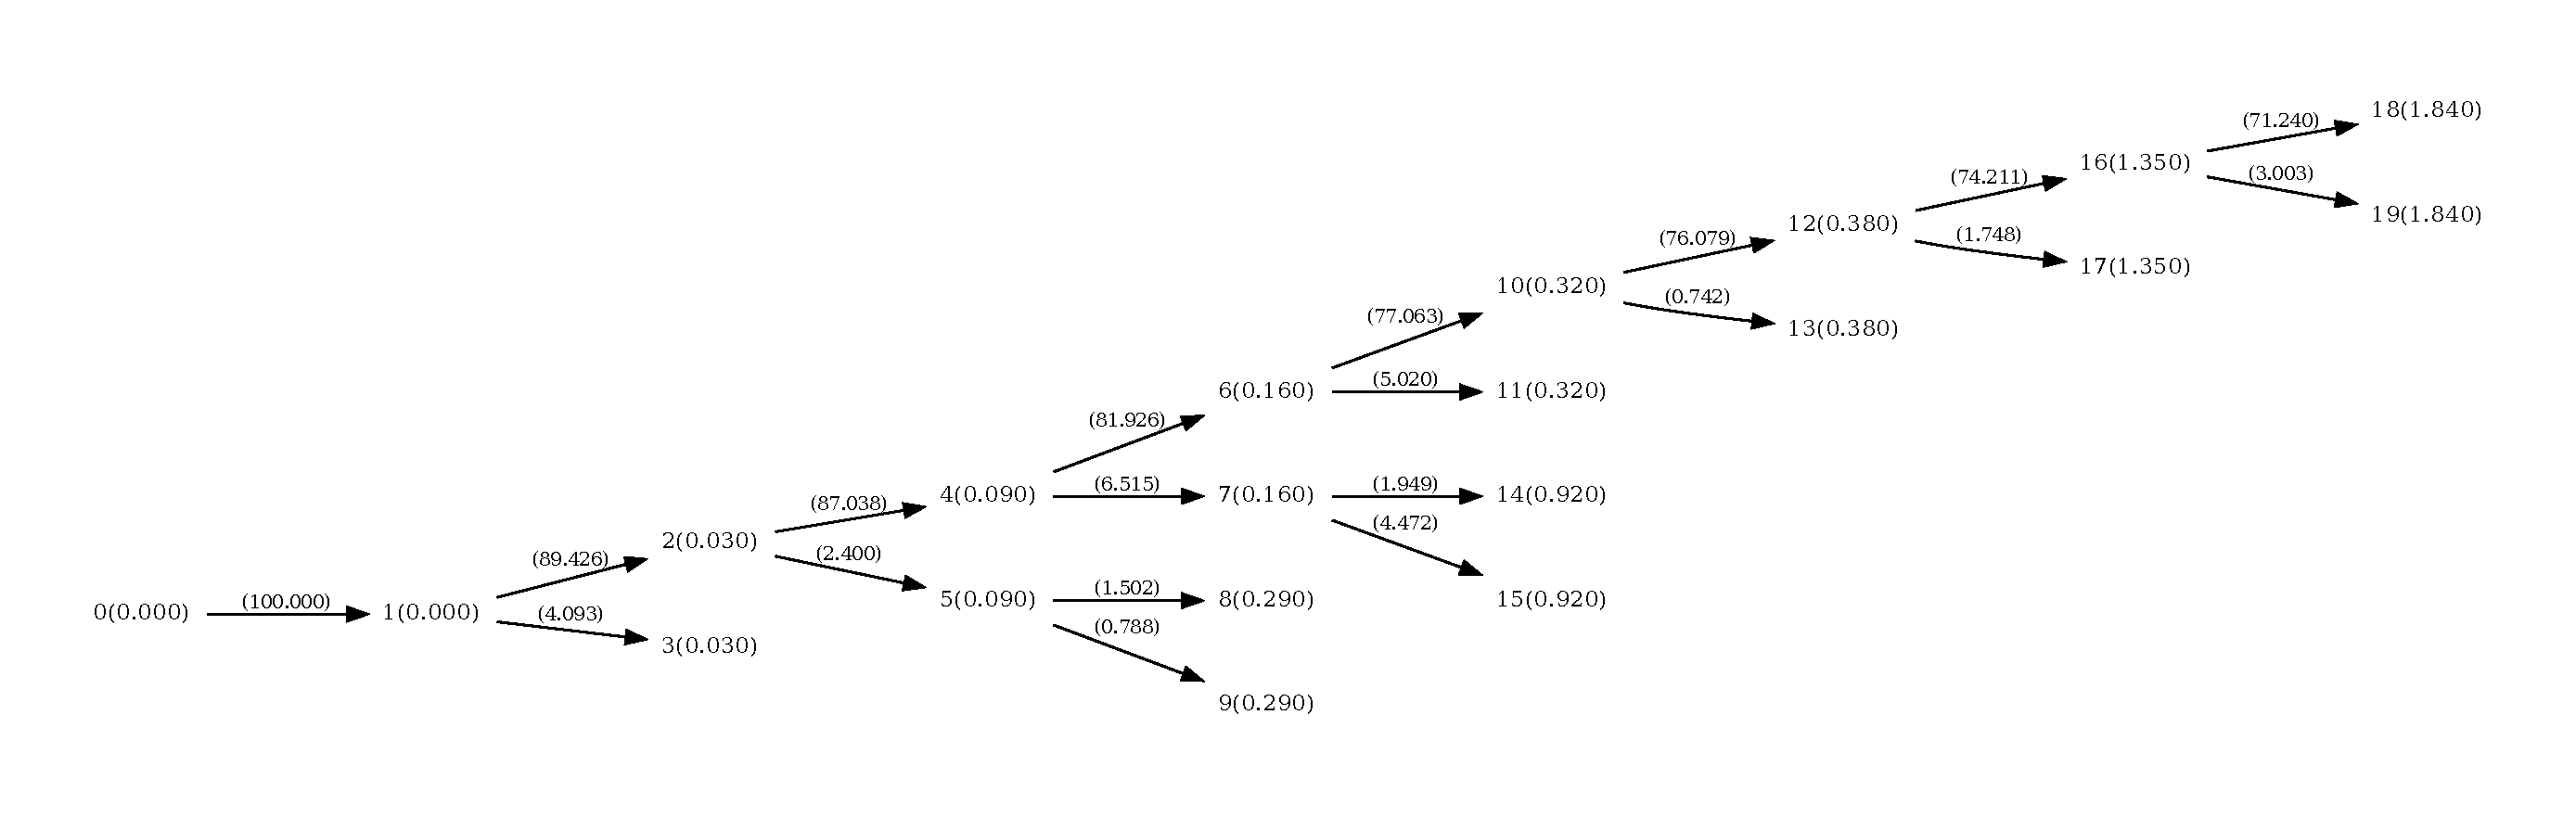
\includegraphics[width=1.2\textwidth]{./sample_jet_graph/graph-Matter/Jet_Matter.pdf}
\onslide<3>
\includegraphics[width=6.\textwidth]{./sample_jet_graph/graph-Martini/Jet_Martini.pdf}
\end{overprint}
\end{figure}
\end{center}
\end{frame}

\begin{frame}{Use jetscape framework}
\begin{columns}
\begin{column}{0.3\textwidth}
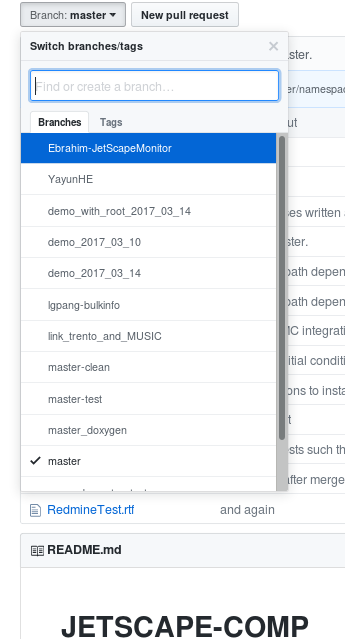
\includegraphics[width=\textwidth]{branches.png}
\end{column}
\begin{column}{0.7\textwidth}
\begin{itemize}
\item Currently, the repo is a little messy. The official JETSCAPE 1.0 is still under developing. 
\item We have many transport modules: parton cascade model, Diffusion (Fortran/C++), Heavy quark linear Boltzmann equation (C++).
\item Use this environment to connect among these and to other models.
\end{itemize}
\end{column}
\end{columns}


\end{frame}

\end{document}
